\documentclass[11pt, a4paper]{article}

\usepackage{amsmath}
\usepackage{amssymb}
\usepackage{graphicx}
\usepackage{listings}
\usepackage{color}
\usepackage[section]{placeins}
\usepackage{paralist}
\usepackage{fullpage}
\usepackage{glossaries}
\usepackage{url}

\usepackage{caption}
\usepackage{subcaption}

\newcommand*{\titleGM}{\begingroup
\hbox{ 
\hspace*{0.2\textwidth} 
\rule{1pt}{\textheight} 
\hspace*{0.05\textwidth} 
\parbox[b]{0.75\textwidth}{ 

{\noindent\Huge\bfseries An Android Homepage Widget}\\[2\baselineskip] % Title
{\large \textit{SEM2220 Assignment 3}}\\[4\baselineskip] % Tagline or further description
{\Large \textsc{Alexander D Brown (adb9)}} % Author name

\vspace{0.5\textheight} 
}}
\endgroup}


\begin{document}
\titleGM 
\tableofcontents
\newpage

\section{Introduction}
This report details the process undertaken to produce an Android widget based 
on the existing code to load sessions from a SQLite database. This widget had 
several requirements, including the ability to select different days from the 
database as well as provide notifications read from a remote URL.

\section{Design}
The widget was designed in accordance with the Android App Widget Design 
Guidelines\cite{google2013widget}, which define guides for design constraints 
like the minimum and maximum size of the widget, layouts and backgrounds, etc.

To help conform to these guidelines, the template design 
pack\cite{google2013widgettemplates} provided by the Android Open Source 
Project under the Apache 2 License was used to design the widget. 

A mock version of the widget was created to view how it would appear on a 
device. From this is became obvious that the widget would need to be four 
cells wide (the maximum) by at least two cells tall.

This size would allow a view with the following information on it:

\begin{itemize}
  \item A title for the Widget
  \item Two buttons, one to move backwards through days and one to move forward
        through days
  \item A list of the sessions available for the specified day.
  \item The notification loaded from a remote site.
\end{itemize}

To keep the buttons accessible, they were made such that their minimum size was
a single cell each and surrounded the list of sessions to make the flow of data
natural. To conform to the iconography standards\cite{google2013iconography},
another resource was used from the Android Open Source Project; the Action Bar 
Icon Pack\cite{google2013iconpack}.

The notification display was kept small so that it would not obstruct the view
of the data, but so that it would be easy to see at a glance. Finally, the 
title was given colour, based on the recommended 
colours\cite{google2013colour}, a purely aesthetic element.

\begin{figure}[h]
\centering
\begin{subfigure}[h]{0.3\textwidth}
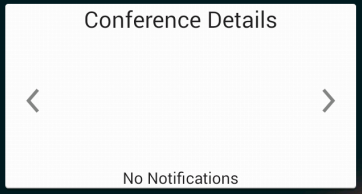
\includegraphics[width=\textwidth]{img/design_initial}
\caption{Initial Widget Design}
\end{subfigure}
\begin{subfigure}[h]{0.3\textwidth}
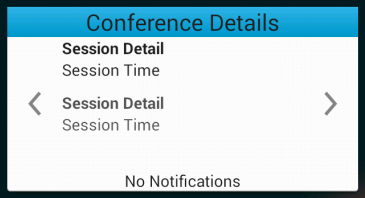
\includegraphics[width=\textwidth]{img/design_second}
\caption{Improved Widget Design}
\end{subfigure}
\begin{subfigure}[h]{0.3\textwidth}
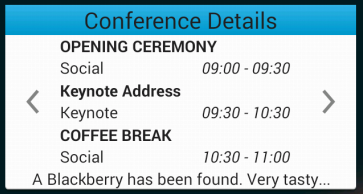
\includegraphics[width=\textwidth]{img/design_final}
\caption{Final Widget Design}
\end{subfigure}

\caption{Evolution of the Widget Design}
\label{fig:widget_design}
\end{figure}

Figure~\ref{fig:widget_design} shows the evolution of the design for the 
widget.

\section{Development}


\section{Testing}


\section{Evaluation}


Breaking down the mark scheme the author has predicted the grade which should 
be given for each part, this is shown in table~\ref{tab:marks}.

Therefore, the author feels a mark of 82\% should be awarded. The values chosen 
were based on the following reasons:

\begin{description}
\item[Documentation] 
\item[Implementation] 
\item[Flair] 
\item[Testing] 
\end{description}

\begin{table}[h]
\centering
\begin{tabular}{|c|c|c|}\hline
\textbf{Part} & \textbf{Worth} & \textbf{Predicted Grade} \\ \hline
Documentation & 30\% & 25\% \\ 
Implementation & 50\% & 45\% \\ 
Flair & 10\% & 5\% \\ 
Testing & 10\% & 7\% \\ \hline
Total & 100\% & 82\% \\ \hline
\end{tabular}
\caption{Break Down of Marks}\label{tab:marks}
\end{table}

\newpage

\bibliographystyle{IEEEtran}
\bibliography{bibliography}

\end{document}
